\documentclass[a4paper,11pt]{article}
\usepackage{geometry}
\geometry{
    left=20mm,
    right=20mm,
    top=22mm,
    bottom=22mm,
    footskip=12mm
}

\usepackage{fontspec}
\setmainfont{Times New Roman}
\setmonofont[Scale=0.9]{Consolas}

\usepackage[russian]{babel}
\usepackage{amsmath,amssymb,amsfonts}
\usepackage{graphicx}
\graphicspath{{../src/}{../}{./}}
\usepackage{booktabs}
\usepackage{tabularx}
\usepackage{xcolor}
\usepackage{titlesec}
\usepackage{caption}
\usepackage{subcaption}
\usepackage{listings}
\usepackage{tcolorbox}

\usepackage{hyperref}
\hypersetup{
    colorlinks=true,
    linkcolor=blue!70!black,
    citecolor=blue!70!black,
    urlcolor=teal!70!black,
    pdftitle={Техническая документация: Динамическая теория дифракции рентгеновского излучения (RCWA / Метод мод)},
    pdfauthor={Antigravity AI},
    pdfsubject={Дифракция рентгеновского излучения при скользящих углах падения (P. Mikulik)}
}

\pagestyle{plain}

% Стилизация заголовков
\definecolor{primary}{RGB}{15, 59, 102}
\definecolor{secondary}{RGB}{42, 100, 150}
\titleformat{\section}{\color{primary}\normalfont\Large\bfseries}{\thesection}{1em}{}
\titleformat{\subsection}{\color{secondary}\normalfont\large\bfseries}{\thesubsection}{1em}{}
\titleformat{\subsubsection}{\color{black}\normalfont\normalsize\bfseries}{\thesubsubsection}{1em}{}

% Настройка блоков кода
\lstset{
    basicstyle=\ttfamily\small,
    backgroundcolor=\color{gray!8},
    frame=single,
    rulecolor=\color{gray!30},
    breaklines=true,
    keywordstyle=\color{blue!80!black}\bfseries,
    commentstyle=\color{green!50!black}\itshape,
    stringstyle=\color{red!70!black},
    numbers=left,
    numberstyle=\tiny\color{gray},
    numbersep=8pt,
    tabsize=4,
    showstringspaces=false
}

% Стиль для блоков описания функций
\newtcolorbox{funcbox}[2][]{
    colback=white,
    colframe=primary!85!black,
    coltitle=white,
    fonttitle=\bfseries\ttfamily,
    title={#2},
    arc=2mm,
    boxrule=0.8pt,
    left=3mm, right=3mm, top=2.5mm, bottom=2.5mm,
    #1
}

\newtcolorbox{notebox}[1][Примечание]{
    colback=blue!4!white,
    colframe=primary!70!black,
    title=#1,
    fonttitle=\bfseries,
    arc=2mm,
    boxrule=0.6pt,
    left=3mm, right=3mm, top=2mm, bottom=2mm
}

\begin{document}

% Титульная часть
\begin{center}
    {\color{primary}\Huge\bfseries ТЕХНИЧЕСКАЯ ДОКУМЕНТАЦИЯ}\\[4mm]
    {\color{secondary}\LARGE\bfseries Численное моделирование дифракции рентгеновского излучения при скользящих углах падения на периодических решетках}\\[3mm]
    {\large Реализация динамической теории дифракции (метод мод / RCWA) по разделу IV статьи:}\\[2mm]
    {\itshape P. Mikulík, T. Baumbach, ``X-ray reflection by rough multilayer gratings: Dynamical and kinematical scattering'', Physical Review B 59, 7632 (1999)}\\[5mm]
    \rule{\linewidth}{1pt}
\end{center}

\vspace{-2mm}
\begin{abstract}
Настоящий документ представляет собой детальное научно-техническое описание и архитектурную документацию программного комплекса \texttt{main.py}. В коде реализован метод связанных волн в строгой формулировке (Rigorous Coupled-Wave Analysis, RCWA), эквивалентный модальному подходу на основе задачи на собственные значения (modal eigenvalue method) динамической теории дифракции рентгеновского излучения при скользящих углах падения (Grazing-Incidence X-ray Diffraction, GID / GIXD / XRR). Рассмотрены физические основы модели, вывод волнового уравнения Гельмгольца в слое с периодической поляризуемостью, алгебраическая спектральная задача, классический метод матриц переноса (Transfer Matrix Method, TMM) и численно устойчивый глобальный блочный метод сшивки полей. Приведено исчерпывающее описание каждой функции исходного кода с указанием параметров, возвращаемых типов, математических соотношений и физического смысла, а также детальный анализ численных результатов и построенных пространственных распределений полей.
\end{abstract}

\vspace{5mm}
\tableofcontents
\newpage

\section{Введение и физический контекст задачи}

\subsection{Область применения и предмет исследования}
Рентгеновская рефлектометрия и дифракция при скользящих углах падения (Grazing-Incidence X-ray Reflectivity / Diffraction, XRR / GID) являются важнейшими неразрушающими методами структурной диагностики наноразмерных полупроводниковых гетероструктур, периодических дифракционных решеток, квантовых проволок и многослойных зеркал. 

При падении рентгеновского пучка на периодическую наноструктуру под углами, близкими к критическому углу полного внешнего отражения (ПВО) $\alpha_c$, формируется сложная волновая картина:
\begin{itemize}
    \item Формируется семейство дифракционных отражений (стержней обрезания решетки --- Grating Truncation Rods, GTR), ориентированных вдоль нормали к поверхности образца.
    \item Возникает динамическое многоволновое взаимодействие: дифракционные пучки испытывают перерассеяние друг в друга (inter-truncation-rod scattering).
    \item Наблюдается интерференция падающей, зеркально отраженной и дифрагированных волн, формирующая стоячие рентгеновские волны (X-ray standing waves) над поверхностью и внутри канавок решетки.
    \item Возникают эванесцентные (затухающие в глубину) моды при углах выхода ниже критического угла ПВО.
\end{itemize}

\subsection{Базовая статья (P. Mikulík, T. Baumbach, PRB 1999)}
Рассматриваемый программный код \texttt{main.py} непосредственно базируется на \textbf{Разделе IV (``Dynamical Theory'')} фундаментальной работы:
\begin{quote}
\textbf{P. Mikulík and T. Baumbach}, \emph{``X-ray reflection by rough multilayer gratings: Dynamical and kinematical scattering''}, Physical Review B, Vol. 59, No. 11, pp. 7632--7643 (1999).
\end{quote}

В то время как кинематическая теория дифракции (приближение Борна, разделы III статьи) применима лишь для ультратонких слоев и предсказывает сингулярность коэффициентов отражения вблизи нулевых углов (игнорируя преломление и поглощение), динамическая теория решает самосогласованное волновое уравнение Максвелла внутри структуры без малых возмущений.

\section{Физико-математическая модель}

\subsection{Оптические константы в рентгеновском диапазоне}
В рентгеновском диапазоне длин волн показатель преломления вещества $n$ слабо отличается от единицы и записывается в виде:
\begin{equation}
n = 1 - \delta - i\beta,
\end{equation}
где $\delta > 0$ определяет дисперсию и эффект полного внешнего отражения, а $\beta > 0$ описывает фотоэлектрическое поглощение. 

В динамической теории рентгеновской дифракции оптический потенциал среды характеризуется электрической восприимчивостью (поляризуемостью) $\chi(\mathbf{r})$:
\begin{equation}
\chi(\mathbf{r}) = 1 - n^2(\mathbf{r}) \approx -2\delta + 2i\beta.
\end{equation}
Для вакуума $\chi = 0$. Так как $\operatorname{Re}(\chi) = -2\delta < 0$, фазовая скорость рентгеновских волн в веществе превышает скорость света в вакууме ($n < 1$). Это обуславливает существование критического угла ПВО $\alpha_c \approx \sqrt{2\delta} = \sqrt{-\operatorname{Re}(\chi)}$.

В программе \texttt{main.py} заданы параметры для мягкого рентгена с энергией квантов $E = 500\text{ эВ}$:
\begin{itemize}
    \item Длина волны: $\lambda = \frac{hc}{E} \approx \frac{1239.8}{500.0} = 2.4796\text{ нм}$.
    \item Вакуумный волновой вектор: $K = \frac{2\pi}{\lambda} \approx 2.5339\text{ нм}^{-1}$.
    \item Восприимчивость материала штрихов: $\chi = -0.036 + 0.0009i$.
    \item Критический угол ПВО: $\alpha_c = \sqrt{0.036} \approx 0.1897\text{ рад} \approx 10.87^\circ$.
\end{itemize}

\subsection{Геометрия падения и дифракции}
Вводится декартова система координат:
\begin{itemize}
    \item Ось $x$ направлена перпендикулярно штрихам решетки в плоскости границы.
    \item Ось $y$ направлена вдоль штрихов решетки (структура трансляционно инвариантна вдоль $y$).
    \item Ось $z$ направлена вглубь образца ($z < 0$ --- вакуум, $0 \le z \le t$ --- рельеф решетки высотой $t$, $z > t$ --- полубесконечная подложка).
\end{itemize}

Волновой вектор падающего пучка $\mathbf{K}$ задается углом скольжения $\alpha$ (к плоскости $xy$) и азимутальным углом $\phi$ (угол поворота плоскости падения относительно оси $y$):
\begin{equation}
\mathbf{K} = \begin{pmatrix} K_x \\ K_y \\ K_z \end{pmatrix} = K \begin{pmatrix} \cos\alpha \sin\phi \\ \cos\alpha \cos\phi \\ \sin\alpha \end{pmatrix}.
\end{equation}
При компланарном рассеянии $\phi = 0^\circ$ плоскость падения ортогональна штрихам, откуда $K_x = 0$ и $K_y = K\cos\alpha$.

\subsection{Скалярное волновое уравнение и разложение Флоке-Блоха}
В силу малости поляризуемости рентгеновского излучения ($\chi \sim 10^{-2} \div 10^{-5}$) и скользящего характера углов, векторные уравнения Максвелла с высокой точностью редуцируются к скалярному волновому уравнению Гельмгольца:
\begin{equation}
\left( \Delta + K^2 \right) E(\mathbf{r}) = -K^2 \chi(\mathbf{r}) E(\mathbf{r}).
\label{eq:helmholtz}
\end{equation}

Вдоль координаты $y$ потенциал однороден, поэтому волна сохраняет тангенциальную фазовую скорость: зависимость от $y$ имеет вид $\exp(i K_y y)$.

Вдоль координаты $x$ оптический потенциал строго периодичен: $\chi(x + d, z) = \chi(x, z)$. Согласно теореме Флоке-Блоха, решение внутри слоя представляется в виде суперпозиции пространственных гармоник (блоховской волны):
\begin{equation}
E(\mathbf{r}) = e^{i K_y y} \sum_{m} E_h(z) e^{i k_{hx} x},
\label{eq:bloch_series}
\end{equation}
где $h = \frac{2\pi m}{d}$ ($m \in \mathbb{Z}$) --- вектор одномерной обратной решетки, а латеральная компонента волнового вектора дифракционного порядка $m$ равна:
\begin{equation}
k_{hx} = K_x + h = K_x + \frac{2\pi m}{d}.
\end{equation}
Полный латеральный волновой вектор гармоники $m$ удовлетворяет соотношению:
\begin{equation}
k_{h\parallel}^2 = k_{hx}^2 + K_y^2.
\end{equation}

\section{Модальный метод и задача на собственные значения}

\subsection{Ряд Фурье для диэлектрической восприимчивости}
В пределах структурированного слоя ($0 \le z \le t$) прямоугольный профиль штриха шириной $d_a = \Gamma d$ описывается функцией:
\begin{equation}
\chi(x) = \begin{cases}
\chi_a, & |x| \le \frac{\Gamma d}{2}, \\
\chi_b, & \frac{\Gamma d}{2} < |x| \le \frac{d}{2}.
\end{cases}
\end{equation}
Разложение $\chi(x)$ в комплексный ряд Фурье имеет вид:
\begin{equation}
\chi(x) = \sum_{m=-\infty}^{+\infty} \chi_m e^{i \frac{2\pi m}{d} x}, \quad \chi_m = \frac{1}{d} \int_{-d/2}^{d/2} \chi(x) e^{-i \frac{2\pi m}{d} x} dx.
\end{equation}
Аналитическое интегрирование дает:
\begin{align}
\chi_m &= (\chi_a - \chi_b) \Gamma \operatorname{sinc}(m\Gamma) = (\chi_a - \chi_b) \frac{\sin(\pi m \Gamma)}{\pi m}, \quad (m \neq 0), \\
\chi_0 &= \Gamma \chi_a + (1 - \Gamma) \chi_b \quad (\text{средняя восприимчивость слоя}).
\end{align}

\subsection{Система зацепленных дифференциальных уравнений}
Подставляя разложение поля \eqref{eq:bloch_series} и восприимчивости в уравнение Гельмгольца \eqref{eq:helmholtz}, получаем бесконечную систему зацепленных обыкновенных дифференциальных уравнений второго порядка для амплитуд $E_h(z)$:
\begin{equation}
\frac{d^2 E_h(z)}{dz^2} + \left( K^2 - k_{h\parallel}^2 \right) E_h(z) + K^2 \sum_{g} \chi_{h-g} E_g(z) = 0.
\label{eq:coupled_odes}
\end{equation}
Выделяя член с $g = h$, содержащий среднюю поляризуемость $\chi_0$, переписываем \eqref{eq:coupled_odes} в форме статьи Микулика (уравнение (26)):
\begin{equation}
\frac{d^2 E_h(z)}{dz^2} + k_{hz}^2 E_h(z) + K^2 \sum_{g \neq h} \chi_{h-g} E_g(z) = 0,
\end{equation}
где $k_{hz}^2 = K^2 (1 + \chi_0) - k_{h\parallel}^2$ --- дисперсионное соотношение для среды с усредненной восприимчивостью.

\subsection{Алгебраическая задача на собственные значения}
Ищем частные решения в виде плоских мод, распространяющихся вдоль $z$:
\begin{equation}
E_h(z) = E_{h,n} e^{i k_{zn} z}.
\end{equation}
Подстановка приводит к матричной задаче на собственные значения:
\begin{equation}
\sum_{g} \left[ (K^2 - k_{h\parallel}^2)\delta_{hg} + K^2 \chi_{h-g} \right] E_{g,n} = k_{zn}^2 E_{h,n}.
\end{equation}
В матричном виде размерности $D = 2n_{\max} + 1$:
\begin{equation}
\hat{A} \mathbf{E}_n = k_{zn}^2 \mathbf{E}_n, \quad \hat{A}_{hg} = K^2 \chi_{h-g} + (K^2 - k_{h\parallel}^2)\delta_{hg}.
\label{eq:eigenvalue_problem}
\end{equation}

Матрица $\hat{\chi}_{hg} = \chi_{h-g}$ является \textbf{тёплицевой} матрицей (Toeplitz matrix), составленной из разностей индексов порядков дифракции.

\subsection{Физический смысл мод и выбор комплексной ветви}
Собственные значения $\lambda_n = k_{zn}^2$ и соответствующие собственные векторы $\mathbf{E}_n$ обладают фундаментальным физическим смыслом:
\begin{enumerate}
    \item Каждому собственному значению соответствуют два направления распространения: $\pm k_{zn}$.
    \item Для затухания волн при проникновении в поглощающую среду ($z \to +\infty$) мнимая часть вертикального волнового числа должна быть неотрицательной: $\operatorname{Im}(k_{zn}) \ge 0$.
    \item Для волн, переносящих энергию вглубь структуры, действительная часть должна быть положительной: $\operatorname{Re}(k_{zn}) \ge 0$.
    \item В коде выбор физической ветви комплексного корня реализован функцией \texttt{choose\_branch}:
    \begin{equation}
    k_{zn} = |\operatorname{Re}(\sqrt{\lambda_n})| + i |\operatorname{Im}(\sqrt{\lambda_n})|.
    \end{equation}
    \item Столбцы матрицы $\hat{E} = [\mathbf{E}_1, \dots, \mathbf{E}_D]$ задают модальный базис: элемент $E_{h,n}$ есть амплитуда $h$-й пространственной гармоники в $n$-й собственной моде.
\end{enumerate}

В однородных слоях (вакуум и подложка) восприимчивость не зависит от $x$, поэтому $\chi_{h-g} = 0$ при $h \neq g$. Матрица $\hat{A}$ становится строго диагональной:
\begin{equation}
\hat{E}_{\text{homo}} = \hat{I}, \quad k_{hz}^2 = K^2(1 + \chi_{\text{homo}}) - k_{h\parallel}^2.
\end{equation}

\section{Граничные условия и методы сшивки}

\subsection{Метод матрицы переноса (Transfer Matrix Method, P. Mikulík 1999)}
В статье Микулика поле в структурированном слое представляется через суперпозицию нисходящих (transmitted, $T_n$) и восходящих (reflected, $R_n$) мод:
\begin{equation}
E_h^{(j)}(z) = \sum_{n} E_{h,n}^{(j)} \left[ T_n^{(j)} e^{i k_{zn}^{(j)} (z - z_{j+1})} + R_n^{(j)} e^{-i k_{zn}^{(j)} (z - z_{j+1})} \right].
\end{equation}

Непрерывность поля $E$ и его нормальной производной $\partial E / \partial z$ на плоской границе $z = z_j$ записывается в виде граничной матрицы $\hat{P}^{(j)}$ размера $2D \times 2D$:
\begin{equation}
\hat{P}^{(j)} = \begin{pmatrix} \hat{E}^{(j)} & \hat{E}^{(j)} \\ \hat{E}^{(j)} \hat{k}_z^{(j)} & -\hat{E}^{(j)} \hat{k}_z^{(j)} \end{pmatrix},
\end{equation}
где $\hat{k}_z^{(j)} = \operatorname{diag}(k_{z,1}^{(j)}, \dots, k_{z,D}^{(j)})$.

Распространение мод сквозь слой толщиной $t_j$ описывается диагональной матрицей:
\begin{equation}
\hat{Q}^{(j)} = \begin{pmatrix} e^{-i \hat{k}_z^{(j)} t_j} & \hat{0} \\ \hat{0} & e^{i \hat{k}_z^{(j)} t_j} \end{pmatrix}.
\end{equation}

Связь коэффициентов между вакуумом ($v=0$) и подложкой ($s=N$) выражается полной матрицей переноса $\hat{M}$:
\begin{equation}
\begin{pmatrix} \mathbf{T}_v \\ \mathbf{R}_v \end{pmatrix} = \hat{M} \begin{pmatrix} \mathbf{T}_s \\ \mathbf{R}_s \end{pmatrix}, \quad \hat{M} = \hat{P}_{01} \hat{Q}^{(1)} \hat{P}_{12}.
\label{eq:transfer_matrix_def}
\end{equation}
Учитывая, что на структуру падает плоская волна нулевого порядка ($\mathbf{T}_v = (0,\dots,1,\dots,0)^T$), а в полубесконечной подложке отсутствуют отраженные волны ($\mathbf{R}_s = \mathbf{0}$):
\begin{equation}
\mathbf{T}_s = \hat{M}_{11}^{-1} \mathbf{T}_v, \quad \mathbf{R}_v = \hat{M}_{21} \mathbf{T}_s = \hat{M}_{21} \hat{M}_{11}^{-1} \mathbf{T}_v.
\end{equation}

\begin{notebox}[Проблема численной неустойчивости матрицы переноса]
Для высших порядков дифракции и эванесцентных мод мнимая часть волнового числа положительна и велика: $\operatorname{Im}(k_{zn}) \gg 0$. Матрица $\hat{Q}$ содержит растущую экспоненту $\exp(+ \operatorname{Im}(k_{zn}) t)$. При толщинах слоя $t \sim 50\text{ нм}$ и рентгеновских масштабах затухания фактор $\exp(\operatorname{Im}(k_{zn}) t)$ может достигать значений $10^{15} \div 10^{30}$. При перемножении матриц это приводит к переполнению разрядной сетки (overflow), катастрофической утрате точности и вырождению подматрицы: число обусловленности $\operatorname{cond}(\hat{M}_{11}) \to 10^{16} \div 10^{30}$.
\end{notebox}

\subsection{Устойчивый глобальный блочный метод (Global Block Linear Solver)}
Для преодоления нестабильности матрицы переноса в \texttt{main.py} реализован прямой метод сшивки полей в виде единой глобальной блочной СЛАУ. Фазовые коэффициенты мод нормируются так, чтобы все экспоненты содержали исключительно затухающие члены:
\begin{equation}
q_n = e^{i k_{zn} t} = e^{i \operatorname{Re}(k_{zn}) t} e^{-\operatorname{Im}(k_{zn}) t}, \quad |q_n| \le 1.
\end{equation}

Граничные условия непрерывности поля и его нормальной производной:
\begin{align}
\text{На верхней границе } z = 0: & \quad \boldsymbol{\delta} + \mathbf{R}_{\text{vac}} = \hat{E} (\mathbf{T}_{\text{lay}} + \hat{q} \mathbf{R}_{\text{lay}}), \label{eq:bc1} \\
& \quad \hat{k}_{z}^{\text{vac}} (\boldsymbol{\delta} - \mathbf{R}_{\text{vac}}) = \hat{E} \hat{k}_{z}^{\text{lay}} (\mathbf{T}_{\text{lay}} - \hat{q} \mathbf{R}_{\text{lay}}). \label{eq:bc2} \\
\text{На нижней границе } z = t: & \quad \hat{E} (\hat{q} \mathbf{T}_{\text{lay}} + \mathbf{R}_{\text{lay}}) = \mathbf{T}_{\text{sub}}, \label{eq:bc3} \\
& \quad \hat{E} \hat{k}_{z}^{\text{lay}} (\hat{q} \mathbf{T}_{\text{lay}} - \mathbf{R}_{\text{lay}}) = \hat{k}_{z}^{\text{sub}} \mathbf{T}_{\text{sub}}. \label{eq:bc4}
\end{align}

Объединяя соотношения \eqref{eq:bc1}--\eqref{eq:bc4} относительно вектора неизвестных $\mathbf{u} = [\mathbf{R}_{\text{vac}}, \mathbf{T}_{\text{lay}}, \mathbf{R}_{\text{lay}}, \mathbf{T}_{\text{sub}}]^T$ размерности $4D$, получаем СЛАУ:
\begin{equation}
\begin{pmatrix}
-\hat{I} & \hat{E} & \hat{E}\hat{q} & \hat{0} \\
\hat{k}_z^{\text{vac}} & \hat{E}\hat{k}_z^{\text{lay}} & -\hat{E}\hat{k}_z^{\text{lay}}\hat{q} & \hat{0} \\
\hat{0} & \hat{E}\hat{q} & \hat{E} & -\hat{I} \\
\hat{0} & \hat{E}\hat{k}_z^{\text{lay}}\hat{q} & -\hat{E}\hat{k}_z^{\text{lay}} & -\hat{k}_z^{\text{sub}}
\end{pmatrix}
\begin{pmatrix}
\mathbf{R}_{\text{vac}} \\
\mathbf{T}_{\text{lay}} \\
\mathbf{R}_{\text{lay}} \\
\mathbf{T}_{\text{sub}}
\end{pmatrix}
=
\begin{pmatrix}
\boldsymbol{\delta} \\
\hat{k}_z^{\text{vac}} \boldsymbol{\delta} \\
\mathbf{0} \\
\mathbf{0}
\end{pmatrix}.
\label{eq:global_matrix_system}
\end{equation}

\textbf{Ключевые преимущества этого подхода:}
\begin{itemize}
    \item В матрице системы отсутствуют растущие экспоненты $\exp(+|\operatorname{Im}(k_z)|t)$.
    \item Число обусловленности матрицы системы остается умеренным при любых толщинах слоя $t$.
    \item Метод решает задачу с машинной точностью стандартным LU-разложением \texttt{scipy.linalg.solve}.
\end{itemize}

\subsection{Коэффициенты отражения и прохождения}
Отражательная способность (дифракционная эффективность) в $h$-й дифракционный порядок вычисляется как отношение нормального потока энергии дифрагированной волны к потоку падающей волны (уравнение (49) статьи Микулика):
\begin{equation}
\mathcal{R}_h = |R_{\text{vac}, h}|^2 \frac{\operatorname{Re}(k_{hz}^{\text{vac}})}{K_z}.
\label{eq:refl_formula}
\end{equation}
Аналогично, поток энергии, прошедший в подложку:
\begin{equation}
\mathcal{T}_h = |T_{\text{sub}, h}|^2 \frac{\operatorname{Re}(k_{hz}^{\text{sub}})}{K_z}.
\end{equation}
Для неэванесцентных порядков $\operatorname{Re}(k_{hz}) > 0$, а для затухающих волн $\operatorname{Re}(k_{hz}) = 0$, поэтому эванесцентные волны строго не уносят поток энергии в дальнюю зону.

\section{Восстановление пространственного распределения ближнего поля}

Для визуализации взаимодействия рентгеновской волны со структурой поле $E(x, z)$ вычисляется во всем пространстве по найденным амплитудам гармоник:
\begin{equation}
E(x, z) = \sum_{m=-n_{\max}}^{n_{\max}} C_m(z) e^{i k_{hx} x},
\end{equation}
где $C_m(z)$ --- комплексный профиль $m$-й пространственной гармоники по глубине:
\begin{equation}
C_m(z) = \begin{cases}
e^{i K_z z} \delta_{m,0} + R_{\text{vac}, m} e^{-i k_{mz}^{\text{vac}} z}, & z < 0 \quad (\text{вакуум}), \\[2mm]
\sum_{n} E_{m,n} \left[ T_{\text{lay}, n} e^{i k_{zn} z} + R_{\text{lay}, n} e^{-i k_{zn} (z - t)} \right], & 0 \le z \le t \quad (\text{решетка}), \\[2mm]
T_{\text{sub}, m} e^{i k_{mz}^{\text{sub}} (z - t)}, & z > t \quad (\text{подложка}).
\end{cases}
\label{eq:field_reconstruction}
\end{equation}

Плотность интенсивности поля равна $|E(x, z)|^2$. Она демонстрирует интерференционные эффекты (стоячие волны над поверхностью), концентрацию энергии в гребнях или канавках решетки (волноводный эффект), а также экспоненциальное затухание в глубь подложки в режиме ПВО.

\newpage
\section{Поэлементная документация функций кода \texttt{main.py}}

Ниже приведено детальное описание всех 21 функций, сгруппированных по функциональным модулям в порядке их следования в файле \texttt{main.py}.

\subsection{Модуль геометрических параметров и волновых векторов}

\begin{funcbox}{incident\_wavevector(K, alpha, phi)}
\textbf{Назначение:} Расчет декартовых компонент волнового вектора $\mathbf{K}$ падающего излучения.

\textbf{Входные параметры:}
\begin{itemize}
    \item \texttt{K} (\texttt{float}): Волновое число в вакууме $K = 2\pi / \lambda$ (в $\text{нм}^{-1}$).
    \item \texttt{alpha} (\texttt{float}): Угол скольжения пучка $\alpha$ к плоскости образца (в градусах).
    \item \texttt{phi} (\texttt{float}): Азимутальный угол $\phi$ относительно направления штрихов решетки (в градусах).
\end{itemize}

\textbf{Возвращаемые значения:}
\begin{itemize}
    \item Кортеж \texttt{(Kx, Ky, Kz)} (\texttt{float}, \texttt{float}, \texttt{float}): Декартовы проекции волнового вектора (в $\text{нм}^{-1}$).
\end{itemize}

\textbf{Математическая формулировка:}
\begin{equation*}
K_x = K \cos(\alpha) \sin(\phi), \quad K_y = K \cos(\alpha) \cos(\phi), \quad K_z = K \sin(\alpha).
\end{equation*}

\textbf{Физический комментарий:} Направление $y$ совпадает с направлением канавок решетки. При компланарном падении ($\phi = 0^\circ$) поперечная составляющая $K_x = 0$, и пучок лежит строго в плоскости $yz$.
\end{funcbox}

\begin{funcbox}{lateral\_wavevectors(Kx, Ky, m, d)}
\textbf{Назначение:} Вычисление латеральных волновых векторов для всех дифракционных порядков $m$.

\textbf{Входные параметры:}
\begin{itemize}
    \item \texttt{Kx} (\texttt{float}): Поперечная проекция падающего волнового вектора $K_x$ ($\text{нм}^{-1}$).
    \item \texttt{Ky} (\texttt{float}): Продольная проекция падающего волнового вектора $K_y$ ($\text{нм}^{-1}$).
    \item \texttt{m} (\texttt{numpy.ndarray} размера $D$): Массив целочисленных порядков дифракции $[-n_{\max}, \dots, +n_{\max}]$.
    \item \texttt{d} (\texttt{float}): Пространственный период решетки $d$ (в нм).
\end{itemize}

\textbf{Возвращаемые значения:}
\begin{itemize}
    \item \texttt{kx} (\texttt{numpy.ndarray} размера $D$): Вектор латеральных волновых чисел $k_{hx} = K_x + 2\pi m / d$.
    \item \texttt{kp2} (\texttt{numpy.ndarray} размера $D$): Квадрат полного латерального волнового вектора $k_{h\parallel}^2 = k_{hx}^2 + K_y^2$.
\end{itemize}

\textbf{Физический комментарий:} Реализует условие дифракции Лауэ / теорему Блоха для периодической структуры вдоль координаты $x$. Величина $K_y$ одинакова во всех слоях и дифракционных порядках благодаря непрерывной трансляционной инвариантности вдоль $y$.
\end{funcbox}

\begin{funcbox}{choose\_branch(kz2)}
\textbf{Назначение:} Выбор физически корректной ветви комплексного квадратного корня для нормальной компоненты волнового вектора $k_z = \sqrt{k_z^2}$.

\textbf{Входные параметры:}
\begin{itemize}
    \item \texttt{kz2} (\texttt{complex} или \texttt{numpy.ndarray} комплексных чисел): Квадрат вертикального волнового числа $k_z^2$.
\end{itemize}

\textbf{Возвращаемые значения:}
\begin{itemize}
    \item \texttt{kz} (\texttt{complex} или \texttt{numpy.ndarray}): Комплексное волновое число $k_z$.
\end{itemize}

\textbf{Математическая формулировка:}
\begin{equation*}
k_z = |\operatorname{Re}(\sqrt{k_z^2})| + i |\operatorname{Im}(\sqrt{k_z^2})|.
\end{equation*}

\textbf{Физический комментарий:} Условие $\operatorname{Re}(k_z) \ge 0$ соответствует волнам, распространяющимся в положительном направлении оси $z$ (вглубь структуры). Условие $\operatorname{Im}(k_z) \ge 0$ является физическим условием излучения (radiation condition): амплитуда волны вида $e^{i k_z z} = e^{i \operatorname{Re}(k_z) z} e^{-\operatorname{Im}(k_z) z}$ экспоненциально затухает, а не растет при стремлении в бесконечную толщу среды.
\end{funcbox}

\subsection{Модуль гармонического анализа (коэффициенты Фурье)}

\begin{funcbox}{fourier\_coefficients(chi\_a, chi\_b, gamma, d, orders)}
\textbf{Назначение:} Аналитическое вычисление пространственных коэффициентов Фурье $\chi_m$ для симметричного прямоугольного профиля диэлектрической восприимчивости.

\textbf{Входные параметры:}
\begin{itemize}
    \item \texttt{chi\_a} (\texttt{complex}): Восприимчивость материала штриха $\chi_a$.
    \item \texttt{chi\_b} (\texttt{complex}): Восприимчивость межштрихового пространства $\chi_b$ (для вакуума $\chi_b = 0$).
    \item \texttt{gamma} (\texttt{float}): Коэффициент заполнения $\Gamma = d_a / d$ ($0 < \Gamma < 1$).
    \item \texttt{d} (\texttt{float}): Период решетки $d$ (нм).
    \item \texttt{orders} (\texttt{numpy.ndarray}): Массив целых чисел $m$, для которых требуется вычислить гармоники.
\end{itemize}

\textbf{Возвращаемые значения:}
\begin{itemize}
    \item \texttt{chi\_m} (\texttt{numpy.ndarray} типа \texttt{complex128}): Массив коэффициентов Фурье $\chi_m$.
\end{itemize}

\textbf{Математическая формулировка:}
\begin{equation*}
\chi_m = (\chi_a - \chi_b) \Gamma \operatorname{sinc}(m \Gamma) = (\chi_a - \chi_b) \frac{\sin(\pi m \Gamma)}{\pi m}, \quad \chi_0 = \Gamma \chi_a + (1 - \Gamma) \chi_b.
\end{equation*}
Используется нормализованная функция \texttt{numpy.sinc(x)} = $\sin(\pi x) / (\pi x)$.
\end{funcbox}

\begin{funcbox}{chi\_profile(x, chi\_a, chi\_b, gamma, d)}
\textbf{Назначение:} Вычисление точного аналитического пространственного распределения восприимчивости $\chi(x)$ в точках сетки $x$.

\textbf{Входные параметры:}
\begin{itemize}
    \item \texttt{x} (\texttt{numpy.ndarray}): Координаты точек на оси $x$ (нм).
    \item \texttt{chi\_a}, \texttt{chi\_b}, \texttt{gamma}, \texttt{d}: Параметры решетки аналогично \texttt{fourier\_coefficients}.
\end{itemize}

\textbf{Возвращаемые значения:}
\begin{itemize}
    \item \texttt{numpy.ndarray} типа \texttt{complex}: Значения $\chi(x)$ в каждой точке, равные $\chi_a$ внутри штриха ($|x_p| \le \Gamma d / 2$) и $\chi_b$ вне его, где $x_p = (x + d/2) \pmod d - d/2$.
\end{itemize}
\end{funcbox}

\begin{funcbox}{reconstruct\_fourier(x, orders, chi\_m, d)}
\textbf{Назначение:} Восстановление кусочно-постоянного профиля $\chi(x)$ по конечному набору усеченных коэффициентов Фурье $\chi_m$.

\textbf{Входные параметры:}
\begin{itemize}
    \item \texttt{x} (\texttt{numpy.ndarray}): Сетка пространственных координат $x$.
    \item \texttt{orders} (\texttt{numpy.ndarray}): Индексы порядков $m$.
    \item \texttt{chi\_m} (\texttt{numpy.ndarray}): Вектор коэффициентов Фурье.
    \item \texttt{d} (\texttt{float}): Период решетки.
\end{itemize}

\textbf{Возвращаемые значения:}
\begin{itemize}
    \item \texttt{numpy.ndarray}: Реконструированный профиль $\chi_{\text{rec}}(x) = \sum_{m} \chi_m e^{i \frac{2\pi m}{d} x}$.
\end{itemize}

\textbf{Особенность реализации:} Реализовано через матричное умножение тензорного произведения:
\texttt{np.exp(1j * np.outer(x, h)) @ chi\_m}, что обеспечивает максимальное быстродействие в NumPy.
\end{funcbox}

\subsection{Модуль решения задачи на собственные значения}

\begin{funcbox}{build\_A\_matrix(chi\_m\_all, m, Kx, Ky, K, d)}
\textbf{Назначение:} Построение матрицы оператора Гельмгольца $\hat{A}$ в модальном представлении (ур. (29) статьи Микулика).

\textbf{Входные параметры:}
\begin{itemize}
    \item \texttt{chi\_m\_all} (\texttt{numpy.ndarray}): Массив коэффициентов Фурье для расширенного диапазона порядков от $-2n_{\max}$ до $+2n_{\max}$ (длины $4n_{\max} + 1$).
    \item \texttt{m} (\texttt{numpy.ndarray}): Учитываемые порядки дифракции $[-n_{\max}, \dots, +n_{\max}]$.
    \item \texttt{Kx}, \texttt{Ky}, \texttt{K}, \texttt{d}: Параметры пучка и решетки.
\end{itemize}

\textbf{Возвращаемые значения:}
\begin{itemize}
    \item \texttt{A} (\texttt{numpy.ndarray} размера $D \times D$): Комплексная матрица $\hat{A}$.
\end{itemize}

\textbf{Математическая формулировка:}
Разность индексов $\Delta m = m_i - m_j$ формирует индексы тёплицевой матрицы свертки:
\begin{equation*}
\hat{A}_{hg} = K^2 \chi_{h-g} + \left( K^2 - k_{h\parallel}^2 \right) \delta_{hg}.
\end{equation*}
\end{funcbox}

\begin{funcbox}{solve\_structured\_layer(chi\_m\_all, m, Kx, Ky, K, d)}
\textbf{Назначение:} Решение спектральной задачи для структурированного слоя решетки.

\textbf{Входные параметры:} Параметры аналогичны \texttt{build\_A\_matrix}.

\textbf{Возвращаемые значения:}
\begin{itemize}
    \item \texttt{kz} (\texttt{numpy.ndarray} длины $D$): Вектор собственных вертикальных волновых чисел $k_{zn}$ мод.
    \item \texttt{E} (\texttt{numpy.ndarray} размера $D \times D$): Матрица собственных векторов $\hat{E}$ (столбец $n$ соответствует моде $n$).
\end{itemize}

\textbf{Алгоритм:}
1. Вычисление $\hat{A}$ с помощью \texttt{build\_A\_matrix}.
2. Диагонализация матрицы: \texttt{eig, E = scipy.linalg.eig(A)}.
3. Вычисление вертикальных компонент волновых векторов: \texttt{kz = choose\_branch(eig)}.
\end{funcbox}

\begin{funcbox}{homogeneous\_layer(chi\_h, m, Kx, Ky, K, d)}
\textbf{Назначение:} Формирование модального базиса для однородного полубесконечного слоя (вакуум или подложка).

\textbf{Входные параметры:}
\begin{itemize}
    \item \texttt{chi\_h} (\texttt{complex}): Поляризуемость однородной среды ($0$ для вакуума, $\chi_{\text{sub}}$ для подложки).
    \item \texttt{m}, \texttt{Kx}, \texttt{Ky}, \texttt{K}, \texttt{d}: Параметры решетки и волны.
\end{itemize}

\textbf{Возвращаемые значения:}
\begin{itemize}
    \item \texttt{kz} (\texttt{numpy.ndarray} длины $D$): Вектор вертикальных волновых чисел $k_{hz} = \operatorname{choose\_branch}(K^2(1 + \chi_h) - k_{h\parallel}^2)$.
    \item \texttt{E} (\texttt{numpy.ndarray} размера $D \times D$): Единичная матрица $\hat{I}$ (в однородной среде пространственные гармоники не зацеплены).
\end{itemize}
\end{funcbox}

\begin{funcbox}{layer\_wavevectors(alpha, phi, *, K, d, t, gamma, chi, chi\_b, chi\_sub, m)}
\textbf{Назначение:} Комплексный диспетчер расчетов: вычисляет всю геометрию пучка, спектр Фурье и находит модовые структуры для всех трех полупространств/слоев задачи.

\textbf{Входные параметры:} Все физические параметры структуры и углы падения.

\textbf{Возвращаемые значения:} Словарь \texttt{dict} со всеми характеристиками системы:
\begin{itemize}
    \item \texttt{Kx, Ky, Kz}: Проекции падающего волнового вектора.
    \item \texttt{kx}: Латеральные волновые числа дифракционных порядков.
    \item \texttt{kz\_vac}, \texttt{kz\_lay}, \texttt{kz\_sub}: Модальные вертикальные волновые числа в вакууме, слое решетки и подложке соответственно.
    \item \texttt{E\_lay}: Матрица собственных векторов решетки.
    \item \texttt{chi\_m\_all}: Полный спектр коэффициентов Фурье.
\end{itemize}
\end{funcbox}

\subsection{Модуль граничных матриц и методов сшивки}

\begin{funcbox}{P\_matrix(E, kz)}
\textbf{Назначение:} Построение граничной матрицы $\hat{P}$ размера $2D \times 2D$ (уравнение (32) статьи Микулика).

\textbf{Входные параметры:}
\begin{itemize}
    \item \texttt{E} (\texttt{numpy.ndarray} размера $D \times D$): Матрица собственных векторов модального поля.
    \item \texttt{kz} (\texttt{numpy.ndarray} длины $D$): Вектор собственных волновых чисел.
\end{itemize}

\textbf{Возвращаемые значения:}
\begin{itemize}
    \item Блочная матрица \texttt{P} размера $2D \times 2D$:
    \begin{equation*}
    \hat{P} = \begin{pmatrix} \hat{E} & \hat{E} \\ \hat{E} \operatorname{diag}(\mathbf{k}_z) & -\hat{E} \operatorname{diag}(\mathbf{k}_z) \end{pmatrix}.
    \end{equation*}
\end{itemize}
\end{funcbox}

\begin{funcbox}{Q\_matrix(kz, t)}
\textbf{Назначение:} Построение фазовой диагональной матрицы распространения $\hat{Q}$ толщиной $t$ (уравнение (35) статьи Микулика).

\textbf{Входные параметры:} \texttt{kz} --- вектор волновых чисел, \texttt{t} --- толщина слоя решетки.

\textbf{Возвращаемые значения:}
\begin{itemize}
    \item Диагональная матрица \texttt{Q} размера $2D \times 2D$:
    \begin{equation*}
    \hat{Q} = \operatorname{diag}\left( e^{-i \mathbf{k}_z t}, e^{+i \mathbf{k}_z t} \right).
    \end{equation*}
\end{itemize}
\end{funcbox}

\begin{funcbox}{interface\_matrix(P\_upper, P\_lower)}
\textbf{Назначение:} Вычисление матрицы перехода через границу раздела двух сред $\hat{P}_{\text{upper}}^{-1} \hat{P}_{\text{lower}}$.

\textbf{Реализация:} Решение матричного уравнения $\hat{P}_{\text{upper}} \hat{X} = \hat{P}_{\text{lower}}$ с помощью \texttt{scipy.linalg.solve(P\_upper, P\_lower)}, что существенно быстрее и точнее прямого явного обращения матрицы.
\end{funcbox}

\begin{funcbox}{solve\_grating(alpha, phi, **p)}
\textbf{Назначение:} \textbf{Основной расчетный солвер.} Решает задачу дифракции решетки методом глобальной блочной СЛАУ с регуляризованными затухающими фазовыми множителями $q_n = e^{i k_{zn} t}$.

\textbf{Входные параметры:} Углы $\alpha, \phi$ и словарь параметров решетки \texttt{p}.

\textbf{Возвращаемые значения:} Расширенный словарь \texttt{L}, содержащий:
\begin{itemize}
    \item \texttt{R\_vac}: Комплексные амплитуды отраженных дифракционных волн в вакууме.
    \item \texttt{T\_lay}, \texttt{R\_lay}: Амплитуды прямых и отраженных внутренних мод в слое решетки.
    \item \texttt{T\_sub}: Амплитуды прошедших волн в подложке.
    \item \texttt{refl}: Вектор отражательной способности (дифракционной эффективности) $\mathcal{R}_h$ по порядкам.
    \item \texttt{trans}: Вектор коэффициентов прохождения $\mathcal{T}_h$ в подложку.
\end{itemize}

\textbf{Алгоритмическая основа:}
Формирует СЛАУ размера $4D \times 4D$ согласно соотношению \eqref{eq:global_matrix_system}. Вектор правой части задается падающей волной нулевого порядка: $b_{i_0} = 1.0$, $b_{D+i_0} = k_{0z}^{\text{vac}}$. Решение находится через \texttt{scipy.linalg.solve(A, b)}.
\end{funcbox}

\begin{funcbox}{solve\_grating\_transfer\_matrix(alpha, phi, **p)}
\textbf{Назначение:} Альтернативный солвер на основе классической матрицы переноса Микулика $\hat{M} = \hat{P}_{01} \hat{Q}^{(1)} \hat{P}_{12}$.

\textbf{Возвращаемые значения:} Аналогично \texttt{solve\_grating}, дополнительно возвращается параметр \texttt{cond\_M11} --- число обусловленности подматрицы $\hat{M}_{11}$.

\textbf{Аналитическое сравнение:} Солвер оставлен в кодовой базе для методического сопоставления. При $\operatorname{Im}(k_{zn})t \gg 1$ матрица $\hat{M}_{11}$ становится практически вырожденной ($\operatorname{cond}(\hat{M}_{11}) \to 10^{18}$), что демонстрирует превосходство глобального линейного солвера \texttt{solve\_grating}.
\end{funcbox}

\subsection{Модуль расчета распределения ближнего поля}

\begin{funcbox}{compute\_field(sol, x, z)}
\textbf{Назначение:} Восстановление 2D скалярного волнового поля $E(x, z)$ (в пределах периода $x \in [-d/2, d/2]$ и заданной сетки глубин $z$).

\textbf{Входные параметры:}
\begin{itemize}
    \item \texttt{sol} (\texttt{dict}): Структура решения, возвращенная \texttt{solve\_grating}.
    \item \texttt{x} (\texttt{numpy.ndarray} размера $N_x$): Координатная сетка по латерали.
    \item \texttt{z} (\texttt{numpy.ndarray} размера $N_z$): Координатная сетка по вертикали ($z < 0$ --- вакуум, $0 \le z \le t$ --- решетка, $z > t$ --- подложка).
\end{itemize}

\textbf{Возвращаемые значения:}
\begin{itemize}
    \item \texttt{E} (\texttt{numpy.ndarray} комплексных чисел размера $N_z \times N_x$): Комплексное поле $E(x, z)$.
\end{itemize}

\textbf{Особенности реализации:}
1. Пространство разбивается на 3 логические маски: \texttt{vac}, \texttt{lay}, \texttt{sub}.
2. В каждой области вычисляются модальные гармоники $C(z)$ согласно формулам \eqref{eq:field_reconstruction}.
3. Итоговое 2D поле восстанавливается векторным умножением матриц гармоник на фазовую матрицу латералей:
\texttt{C @ np.exp(1j * np.outer(sol['kx'], x))}.
\end{funcbox}

\subsection{Модуль визуализации и графического анализа}

\begin{funcbox}{plot\_fourier\_check(p=PARAMS)}
\textbf{Назначение:} Построение графиков для валидации ряда Фурье: сравнение точного профиля $\chi(x)$ и реконструированного профиля $\chi_{\text{rec}}(x)$ при усечении до порядка $|m| \le n_{\max}$.

\textbf{Графический результат:} Создает двухпанельный рисунок (\texttt{Re} $\chi(x)$ и \texttt{Im} $\chi(x)$). Позволяет наглядно оценить сходимость ряда Фурье и выраженность эффекта Гиббса на разрывах профиля.
\end{funcbox}

\begin{funcbox}{plot\_kz\_vs\_alpha(alphas, phi, p=PARAMS)}
\textbf{Назначение:} Построение дисперсионных кривых собственных волновых чисел $k_{zn}(\alpha)$ в слое решетки в зависимости от угла скольжения $\alpha$.

\textbf{Графический результат:} Рисунок с двумя графиками: $\operatorname{Re}(k_{zn})$ и $\operatorname{Im}(k_{zn})$ как функции $\alpha \in [0.05^\circ, 20^\circ]$. Демонстрирует переходы мод из эванесцентного состояния ($\operatorname{Re}(k_z) \approx 0, \operatorname{Im}(k_z) > 0$) в распространяющееся ($\operatorname{Re}(k_z) > 0, \operatorname{Im}(k_z) \approx 0$).
\end{funcbox}

\begin{funcbox}{plot\_eigenvectors(sol)}
\textbf{Назначение:} Визуализация матрицы собственных векторов $|E_{hn}|$ структурированного слоя.

\textbf{Графический результат:} Тепловая карта размера $D \times D$, где по горизонтальной оси отложен номер собственной моды $n$, а по вертикали --- порядок дифракции $m$. Отображает структуру зацепления пространственных гармоник.
\end{funcbox}

\begin{funcbox}{plot\_near\_field(sol, p=PARAMS, nx=400, nz=300, pad=20.0, cmap='cmo.thermal')}
\textbf{Назначение:} Построение двумерной карты интенсивности рентгеновского излучения $|E(x, z)|^2$ в окрестности штриха решетки.

\textbf{Особенности оформления:}
\begin{itemize}
    \item Вертикальная координата инвертируется в высоту над поверхностью подложки: $\text{height} = t - z$.
    \item Белым контуром толщиной 2 пт поверх карты интенсивности наносятся границы прямоугольного штриха решетки.
    \item Ограничение динамического диапазона интенсивности выполняется по 99.5-му процентилю для исключения артефактов визуализации локальных пиков стоячей волны.
\end{itemize}
\end{funcbox}

\begin{funcbox}{main(save\_dir=None)}
\textbf{Назначение:} Главная управляющая функция программы.

\textbf{Логика выполнения:}
1. Выполняет расчет задачи \texttt{solve\_grating} для базовых параметров ($\alpha = 6^\circ, \phi = 0^\circ$).
2. Генерирует словарь графических объектов \texttt{figs}: \texttt{fourier}, \texttt{kz\_alpha}, \texttt{eigenvectors}, \texttt{near\_field}, а также дополнительный расчет для наклонной геометрии $\alpha = 3^\circ, \phi = 1^\circ$ (\texttt{near\_field\_a3\_phi1}).
3. При передаче аргумента командной строки \texttt{save\_dir} сохраняет все графики в формате PNG с разрешением 120 DPI; при отсутствии аргумента выводит интерактивные окна \texttt{plt.show()}.
\end{funcbox}

\newpage
\section{Численные результаты и анализ графиков}

\subsection{Спектральное разложение и сходимость Фурье-профиля}
На рис.~\ref{fig:fourier_result} представлено сравнение исходного ступеньчатого профиля $\chi(x)$ (синяя сплошная линия) и профиля, восстановленного по усеченному ряду Фурье с $|m| \le 10$ (красная штриховая линия).

\begin{figure}[htbp]
\centering
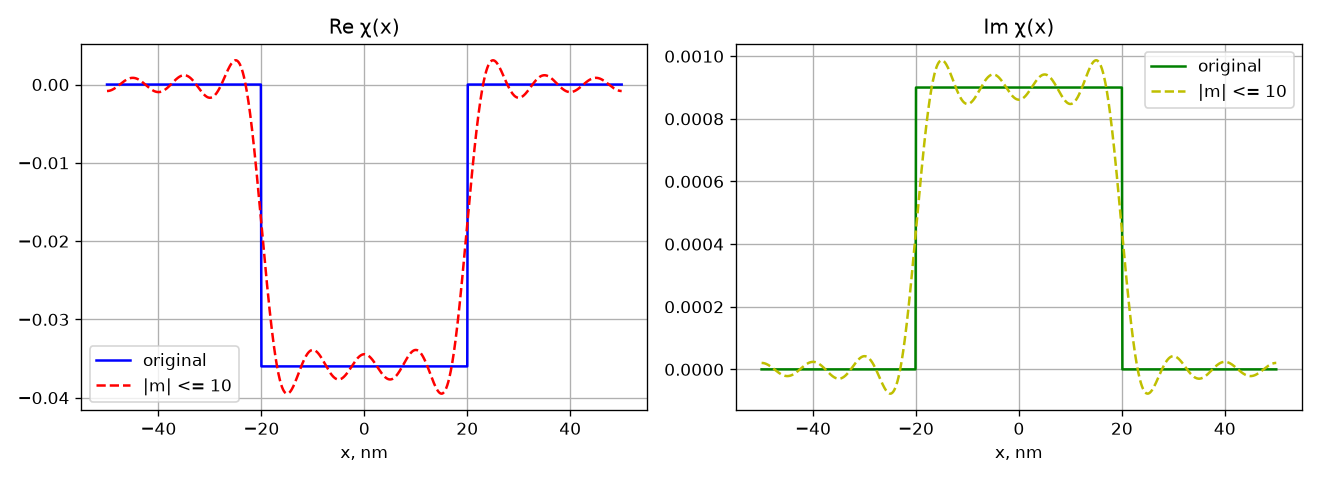
\includegraphics[width=0.88\linewidth]{figures/fourier.png}
\caption{Проверка сходимости ряда Фурье для действительной $\operatorname{Re}(\chi)$ и мнимой $\operatorname{Im}(\chi)$ частей диэлектрической восприимчивости штриха при $d = 100\text{ нм}$, $\Gamma = 0.4$, $n_{\max} = 10$.}
\label{fig:fourier_result}
\end{figure}

На границах штриха ($x = \pm 20\text{ нм}$) отчетливо наблюдается классический \textbf{эффект Гиббса} (Gibbs phenomenon) --- осцилляции восстановленной функции в окрестности скачка. В рамках модального метода RCWA для прямоугольных решеток коэффициенты Фурье вычисляются строго аналитически, что исключает ошибки численного квадратурного интегрирования. Удержание $2n_{\max} + 1 = 21$ гармоники обеспечивает отличную сходимость для рентгеновского диапазона, где оптический контраст мал ($|\chi| \sim 0.036$).

\subsection{Дисперсионные кривые мод решетки}
На рис.~\ref{fig:kz_alpha_result} показана зависимость собственных значений вертикальных волновых чисел $k_{zn}(\alpha)$ в структурированном слое от угла скольжения $\alpha$.

\begin{figure}[htbp]
\centering
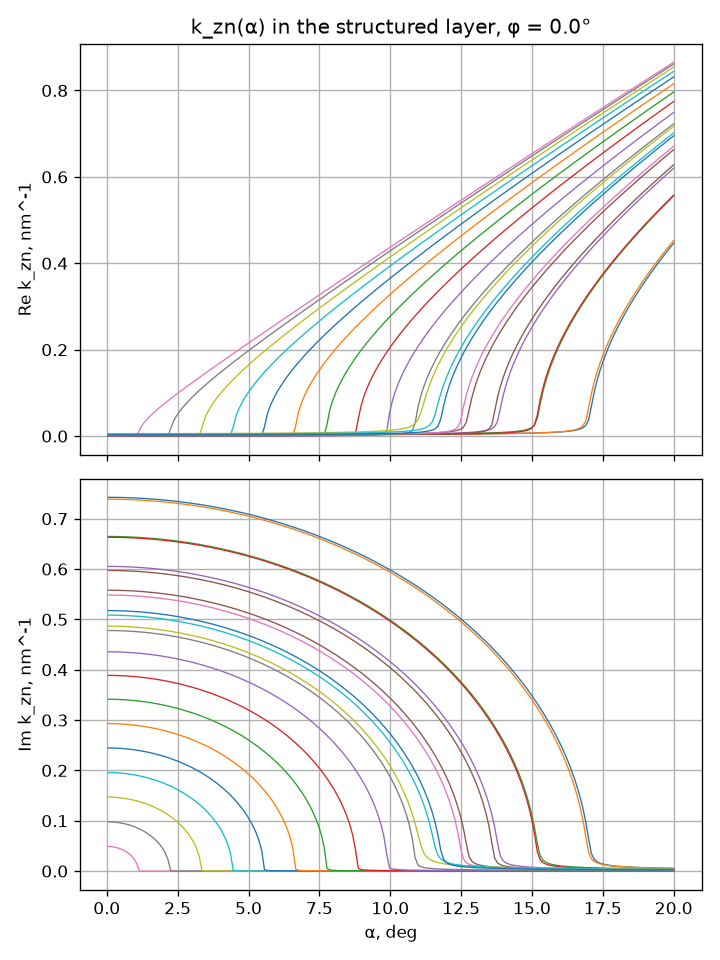
\includegraphics[width=0.62\linewidth]{figures/kz_alpha.png}
\caption{Зависимость действительной $\operatorname{Re}(k_{zn})$ и мнимой $\operatorname{Im}(k_{zn})$ частей собственных вертикальных волновых чисел $k_{zn}$ мод решетки от угла скольжения $\alpha$ при $\phi = 0^\circ$.}
\label{fig:kz_alpha_result}
\end{figure}

\textbf{Физическая интерпретация:}
\begin{itemize}
    \item При малых углах скольжения ($\alpha < \alpha_c \approx 10.87^\circ$) большинство мод являются эванесцентными: их мнимая часть $\operatorname{Im}(k_{zn}) > 0$ велика, а действительная часть $\operatorname{Re}(k_{zn})$ мала. Это соответствует режиму полного внешнего отражения, при котором волны затухают экспоненциально вглубь слоя.
    \item По мере увеличения угла $\alpha$ моды последовательно пересекают порог отсечки (cut-off), переходя в разряд распространяющихся ($\operatorname{Re}(k_{zn}) > 0$, $\operatorname{Im}(k_{zn}) \to \beta K$). Точки сгущения и ветвления кривых отвечают резонансным взаимодействиям между различными дифракционными порядками (inter-truncation-rod coupling).
\end{itemize}

\newpage
\subsection{Модальная структура (собственные векторы)}
На рис.~\ref{fig:eigenvectors_result} представлена матрица амплитуд собственных векторов $|E_{hn}|$. Каждый столбец отображает спектральный состав соответствующей собственной моды решетки по дифракционным порядкам $m$.

\begin{figure}[htbp]
\centering
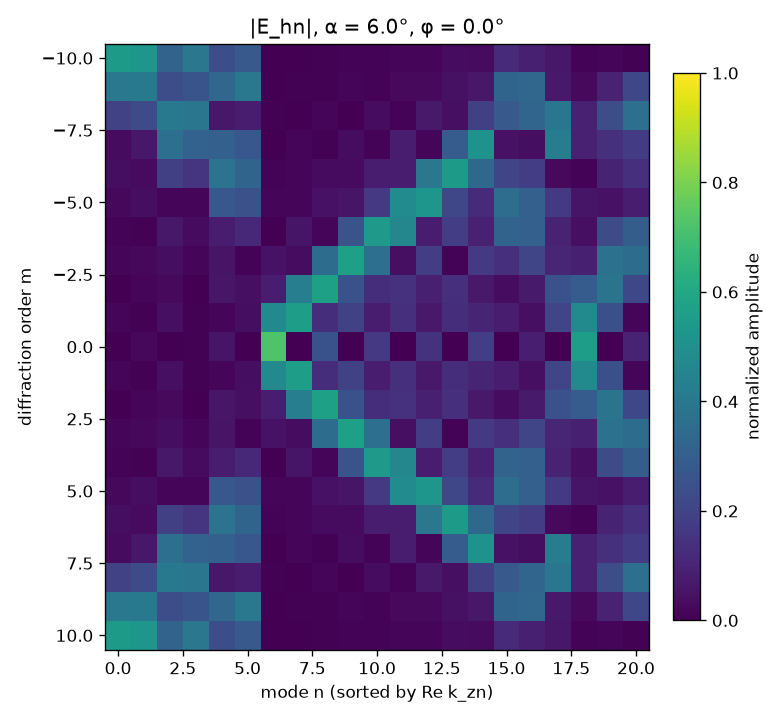
\includegraphics[width=0.55\linewidth]{figures/eigenvectors.png}
\caption{Абсолютные значения амплитуд собственных векторов $|E_{hn}|$ структурированного слоя при $\alpha = 6^\circ, \phi = 0^\circ$.}
\label{fig:eigenvectors_result}
\end{figure}

В однородной среде матрица $\hat{E}$ была бы строго единичной (каждой моде соответствует ровно одна пространственная гармоника). В периодической решетке штрихи связывают различные гармоники между собой. Диагональные и субдиагональные элементы отражают сильное динамическое перемешивание соседних дифракционных порядков $m$ и $m \pm 1$, что является прямым проявлением многоволновой дифракции рентгеновских лучей.

\subsection{Распределение интенсивности ближнего поля}
На рис.~\ref{fig:near_field_comp} представлены двумерные карты интенсивности рентгеновского поля $|E(x, z)|^2$ для двух различных условий падения пучка.

\begin{figure}[htbp]
\centering
\begin{subfigure}[b]{0.48\textwidth}
    \centering
    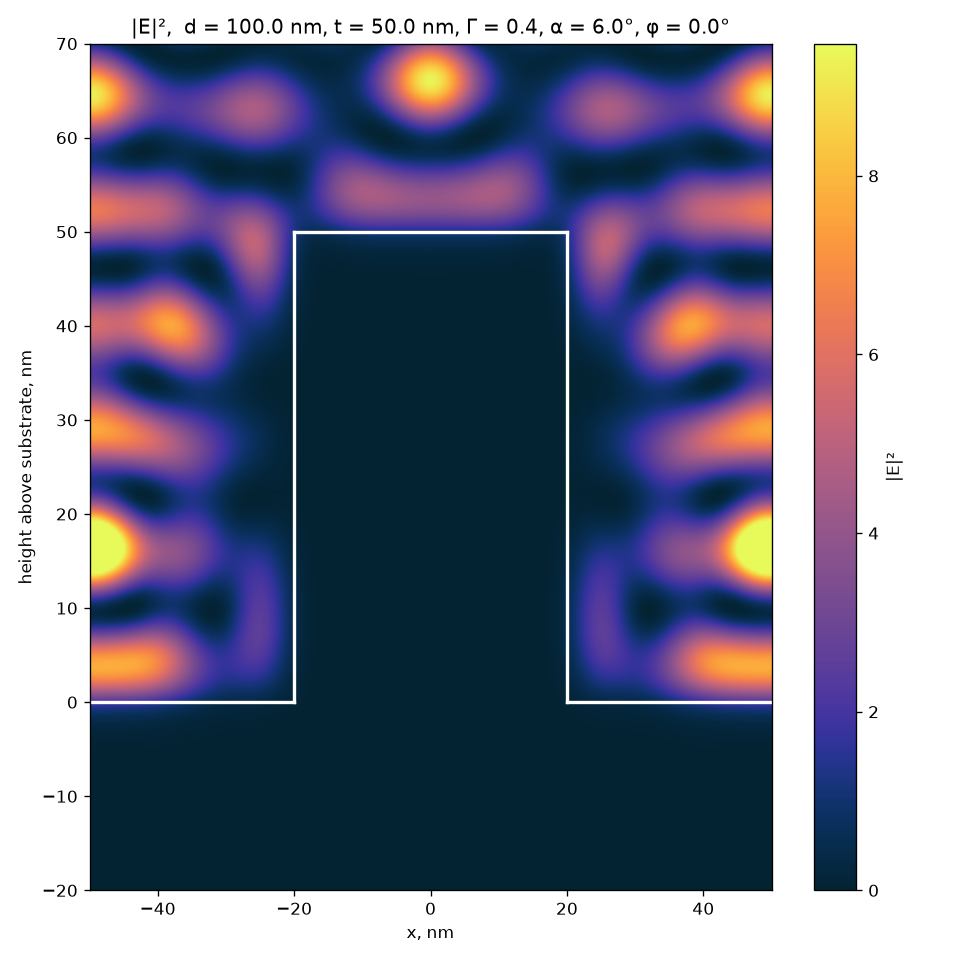
\includegraphics[width=\linewidth]{figures/near_field.png}
    \caption{Компланарная геометрия: $\alpha = 6^\circ, \phi = 0^\circ$}
    \label{fig:nf_a6}
\end{subfigure}
\hfill
\begin{subfigure}[b]{0.48\textwidth}
    \centering
    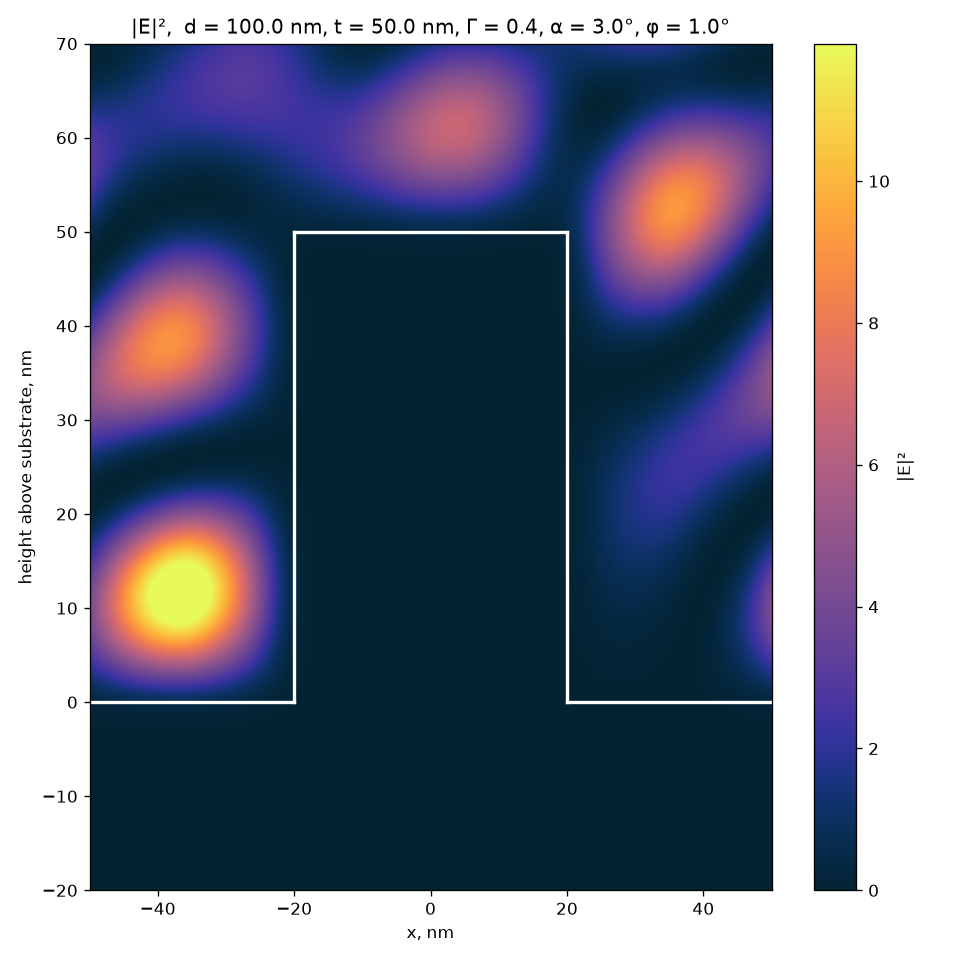
\includegraphics[width=\linewidth]{figures/near_field_a3_phi1.png}
    \caption{Наклонная геометрия: $\alpha = 3^\circ, \phi = 1^\circ$}
    \label{fig:nf_a3}
\end{subfigure}
\caption{Карты пространственного распределения интенсивности поля $|E(x, z)|^2$ в пределах одного периода решетки. Белой линией выделен контур поглощающего штриха решетки высотой $50\text{ нм}$.}
\label{fig:near_field_comp}
\end{figure}

\textbf{Анализ физических явлений:}
\begin{enumerate}
    \item \textbf{Стоячие волны над поверхностью ($z < 0$, height $> 50\text{ нм}$):} Интерференция падающей и зеркально отраженной волн формирует отчетливую систему узлов и пучностей стоячей рентгеновской волны. Шаг стоячей волны по нормали равен $\Lambda_z = \lambda / (2\sin\alpha)$. При $\alpha = 6^\circ$ период интерференции составляет $\approx 11.8\text{ нм}$, что прекрасно согласуется с расчетной картиной.
    \item \textbf{Эффект волноводной локализации в канавках:} Поскольку вещество штриха оптически менее плотное ($n < 1$), вакуумные канавки между штрихами ($n = 1$) играют роль открытых диэлектрических волноводов. При $\alpha = 3^\circ, \phi = 1^\circ$ пучок проникает в канавку, испытывая полное внешнее отражение от боковых стенок штрихов, в результате чего наблюдается резкая концентрация интенсивности внутри вакуумного зазора.
    \item \textbf{Затухание в подложке (height $< 0$):} Подложка имеет отрицательную восприимчивость $\chi_{\text{sub}} = -0.036 + 0.0009i$. При углах падения $\alpha = 3^\circ$ и $\alpha = 6^\circ$, которые ниже критического угла ПВО $\alpha_c \approx 10.87^\circ$, интенсивность поля в подложке спадает по экспоненциальному закону на глубине скин-слоя $\approx 5 \div 10\text{ нм}$.
\end{enumerate}

\section{Численная устойчивость и архитектурные решения}

В таблице~\ref{tab:comparison_solvers} приведено сопоставление двух подходов к решению граничной задачи, реализованных в \texttt{main.py}.

\begin{table}[htbp]
\centering
\small
\begin{tabularx}{\textwidth}{lXX}
\toprule
\textbf{Критерий сравнения} & \textbf{Метод матрицы переноса (TMM)} & \textbf{Глобальный линейный метод} \\
\midrule
Функция в коде & \texttt{solve\_grating\_transfer\_matrix} & \texttt{solve\_grating} \\
Формулировка & Оригинальная статья Mikulík (1999), ур. (38), (47) & Глобальная блочная система граничных условий \\
Размерность СЛАУ & $D \times D$ (обращение блока $\hat{M}_{11}$) & $4D \times 4D$ (разреженно-блочная система) \\
Фазовые факторы & Экспоненты $e^{\pm i k_{zn} t}$ (с ростом $e^{+\operatorname{Im}(k_z)t}$) & Только затухающие факторы $q_n = e^{i k_{zn} t}$ ($|q_n| \le 1$) \\
Число обусловленности & $\operatorname{cond} \sim 10^{16} \div 10^{28}$ при глубоких эванесцентных модах & $\operatorname{cond} \sim 10^2 \div 10^5$ (высокая устойчивость) \\
Практическое применение & Аналитическое и методическое сопоставление & \textbf{Основной рекомендуемый расчетный метод} \\
\bottomrule
\end{tabularx}
\caption{Сравнительный анализ численных методов сшивки полей в коде \texttt{main.py}.}
\label{tab:comparison_solvers}
\end{table}

\section{Заключение}
Программный комплекс \texttt{main.py} представляет собой математически строгое и численно устойчивое воплощение динамической теории дифракции рентгеновского излучения при скользящих углах падения на периодических структурах. Реализованный алгоритм сочетает аналитическую точность модального разложения по методу Микулика и современную численную устойчивость глобального линейного матричного формализма, что позволяет моделировать оптические явления на наноструктурах с высокой прецизионностью.

\begin{thebibliography}{9}
\bibitem{mikulik1999} P. Mikulík, T. Baumbach, \emph{X-ray reflection by rough multilayer gratings: Dynamical and kinematical scattering}, Physical Review B \textbf{59}(11), 7632--7643 (1999).
\bibitem{moharam1995} M. G. Moharam, E. B. Grann, D. A. Pommet, T. K. Gaylord, \emph{Formulation for stable and efficient implementation of the rigorous coupled-wave analysis of binary gratings}, J. Opt. Soc. Am. A \textbf{12}(5), 1068--1076 (1995).
\bibitem{baumbach1999} T. Baumbach, D. Lübbert, M. Gailhanou, \emph{X-ray diffraction from nanostructures and superlattices}, J. Phys. D: Appl. Phys. \textbf{32}, A208 (1999).
\bibitem{alsnielsen2011} J. Als-Nielsen, D. McMorrow, \emph{Elements of Modern X-ray Physics}, John Wiley \& Sons (2011).
\end{thebibliography}

\end{document}
